%!TEX root = ../01-Quantum-Hall-Effect.tex
\chapter{Theoretical Preliminaries}

\section{Two Dimensional Electron Gas (2DEG)}
\begin{figure}
	\centering
	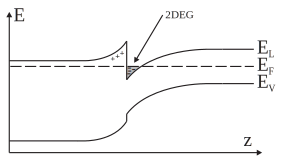
\includegraphics[width=.5\textwidth]{./img/bandstructure-GaAs.pdf}
	\caption[Band structure of AlGaAs-GaAs heterostructure]{\textbf{Band structure of AlGaAs-GaAs heterostructure} The different chemical potentials create a bend in the band edges of the heterostructure, forming a thin, triangular quantum well below the Fermi level}
	\label{fig:bandstructure_GaAs}
\end{figure}
In a two dimensional electron gas, the movement of electrons is confined to a plane, thus leading to quantized levels of motion in the third direction.
For the most problems, these levels can then be ignored.
One way of creating such a 2DEG is the employment of semiconductor-oxide-interfaces.
\autoref{fig:bandstructure_GaAs} shows the band structure of such an AlGaAs-GaAs-junction.
Since the band edges of the materials differ vastly, a thin triangular potential well is formed with its minimum below the Fermi level, effectively confining the electrons to a small region around the junction.
Hence, for low enough temperatures, only the lowest level of the quantum well is occupied and so the motion perpendicular to the junction surface can safely be ignored.
However, the electron still is free to move in a direction parallel to the junction, effectively realizing a 2DEG.

The dispersion relation of a 2DEG is
\begin{equation}\label{eq:subband}
	E_{k_\text{x}, k_\text{y}} = E_0 + \frac{\hbar^2}{2m_\text{eff}}\left(k_\text{x}^2 + k_\text{y}^2\right),
\end{equation}
where $E_0=E_\text{c} + E_\text{s}$ is the sum of the energy of the conduction band and the energy of the quantum well sub-band.

The density of states is calculated by counting the states in k-space
\begin{equation*}
	N(\epsilon) = \underbrace{2}_{\text{spin degeneracy}}\cdot\frac{\pi k^2\cdot S}{4\pi^2} = S\frac{2m_\text{eff}\cdot\epsilon}{2\pi\hbar^2} = S\frac{m_\text{eff}\cdot\epsilon}{\pi\hbar^2}.
\end{equation*}
and differentiating with respect to energy
\begin{equation*}
	\nu(\epsilon) = \frac{1}{S}\cdot\diff[N(\epsilon)]{\epsilon}\theta(\epsilon-E_0) = \frac{m_\text{eff}}{\pi\hbar^2} = \text{const.}.
\end{equation*}

\section{2DEG In a Magnetic Field}
We want to solve the stationary Schrödinger Equation
\begin{equation*}
	\frac{1}{2m_\text{eff}}\left(\vec{p}-e\vec{A}\right)^2\psi = E\psi.
\end{equation*}
In Lorentz gauge, we can choose $\vec{A}=(0, Bx, 0)^T$ and solve by a product ansatz $\psi(x,y,z) = \phi(x,y)Z(z)$.
The z-equation is readily solved with the eigenenergies being the sub-band energies mentioned in \autoref{eq:subband}.
Solving the eigenequation for $\phi(x,y)$ yields the \textit{Landau levels}
\begin{equation*}
	\epsilon_n = \hbar\omega_\text{c}\left(n+\frac{1}{2}\right)\qquad{n\in\mathbb{N}_0},
\end{equation*}
where $\omega_\text{c} = \frac{eB}{m}$ is called the cyclotron frequency.

\section{Experimental Setup}
The experiment is performed inside a two-stage cryostat.
The first stage is thermally insulated from the environment by a dewar flask and multi-layer insulation.
It contains the inner dewar, which is surrounded by a superconducting coil.
During the experiment it is first filled with liquid nitrogen, then purged and filled back with liquid helium.
The second dewar flask forms the probe chamber, a carbon resistor is used to measure the temperature of the inner chamber.
Both chambers are sealed to allow control of the internal pressures and allow recovery of the evaporated helium.
A capillary hole in the inner flask allows liquid helium to transfer to the inner probe chamber.
To further cool the probe chamber below the boiling point of helium at ambient pressure, a vacuum pump can be used to lower the pressure inside the probe chamber.

The variable magnetic field is provided by the aforementioned superconducting coil.
To quickly switch between the normal and persistent operating modes, a superconducting switch is used.
Heating the switch with a resistive heater brings it above its critical temperature, breaking the loop and allowing the current to be adjusted.

An adjustable constant current supply is used to create a current flow through the probes.
The voltage across various test points, spanning the probe longitudinally and transversely, freely selected with two rotary switches, is measured with a multimeter.
An x-y plotter simultaneously records the relationship between the voltage and magnetic field.
